\documentclass[12pt, letterpaper]{article}
\usepackage[titletoc,title]{appendix}
\usepackage{color}
\usepackage{booktabs}
\usepackage[usenames,dvipsnames,svgnames,table]{xcolor}
\definecolor{dark-red}{rgb}{0.75,0.10,0.10}
\definecolor{bluish}{rgb}{0.05,0.05,0.85}

\usepackage[margin=1in]{geometry}
\usepackage[linkcolor=blue,
			colorlinks=true,
			urlcolor=blue,
			pdfstartview={XYZ null null 1.00},
			pdfpagemode=UseNone,
			citecolor={bluish},
			pdftitle={pareto_party}]{hyperref}

\usepackage[resetlabels,labeled]{multibib}
\newcites{SI}{SI References}
\usepackage{natbib}

\usepackage{float}

\usepackage{geometry} % see geometry.pdf on how to lay out the page. There's lots.
\geometry{letterpaper}               % This is 8.5x11 paper. Options are a4paper or a5paper or other... 
\usepackage{graphicx}                % Handles inclusion of major graphics formats and allows use of 
\usepackage{amsfonts,amssymb,amsbsy}
\usepackage{amsxtra}
\usepackage{verbatim}
\setcitestyle{round,semicolon,aysep={},yysep={;}}
\usepackage{setspace}		     % Permits line spacing control. Options are \doublespacing, \onehalfspace
\usepackage{sectsty}		     % Permits control of section header styles
\usepackage{pdflscape}
\usepackage{fancyhdr}		     % Permits header customization. See header section below.
\usepackage{url}                     % Correctly formats URLs with the \url{} tag
\usepackage{fullpage}		%1-inch margins
\usepackage{multirow}
\usepackage{rotating}
\setlength{\parindent}{3em}

\usepackage[T1]{fontenc}
\usepackage[bitstream-charter]{mathdesign}

\usepackage{chngcntr}
\usepackage{booktabs}
\usepackage{longtable}

\def\citeapos#1{\citeauthor{#1}'s (\citeyear{#1})}

\makeatother

\usepackage{footmisc}
\setlength{\footnotesep}{\baselineskip}
\makeatother
\renewcommand{\footnotelayout}{\normalsize \doublespacing}


% Caption
\usepackage[hang, font=small,skip=0pt, labelfont={bf}]{caption}
%\captionsetup[subtable]{font=small,skip=0pt}
\usepackage{subcaption}

% tt font issues
% \renewcommand*{\ttdefault}{qcr}
\renewcommand{\ttdefault}{pcr}

\setcounter{page}{0}

\usepackage{lscape}
\renewcommand{\textfraction}{0}
\renewcommand{\topfraction}{0.95}
\renewcommand{\bottomfraction}{0.95}
\renewcommand{\floatpagefraction}{0.40}
\setcounter{totalnumber}{5}
\makeatletter
\providecommand\phantomcaption{\caption@refstepcounter\@captype}
\makeatother

\title{Pareto Party? Welfare Consequences of Partisanship}

\author{Gaurav Sood\thanks{Gaurav can be reached at, \href{mailto:gsood07@gmail.com}{\texttt{gsood07@gmail.com}}} \and Alex Theodiridis\thanks{Alex can be reached at \href{alexandertheodoridis@gmail.com}{\texttt{alexandertheodoridis@gmail.com}}}}


\begin{comment}

setwd(paste0(githubdir, "pareto_partisan/ms/"))
tools::texi2dvi("pareto_party.tex", pdf = TRUE, clean = TRUE)
setwd(githubdir)

\end{comment}

\begin{document}
\maketitle
\thispagestyle{empty}

\begin{abstract}

\noindent The deepest worry about ``negative'' partisanship is that people will cut their nose to spite their face. Will partisans choose something that isn't Pareto optimal? When offered a choice between a scheme where co-partisans win X and opposing partisans win X + 5 versus where co-partisans win X - 5 and opposing partisans win X - 10, will they opt for the latter?

\end{abstract}

\newpage


\doublespacing

Democrats and Republicans are increasingly sure that they cannot trust the other side. They also increasingly believe that the other side is naive or worse---motivated by bad faith and plausibly even anti-national. Such mistrust poses a grave threat to liberal democracies because it corrodes accountability. Some research suggests that it is indeed true. For instance, data suggest that independents are most responsive to ideological differences and partisans least responsive to ideological differences with co-partisans \citep{sood2018all}. Others cite a more conventional example. Despite any number of missteps by Mr. Trump, well north of 80\% of Republicans approve of him.\footnote{\href{https://news.gallup.com/poll/203198/presidential-approval-ratings-donald-trump.aspx}{https://news.gallup.com/poll/203198/presidential-approval-ratings-donald-trump.aspx}}

Reduced accountability is one thing. Spiteful choices are another. We find that partisans do not choose what is Pareto optimal but are willing to take a hit to their payoff to reduce payoffs for the other side.

There is a long literature \citep{amira2019group}.

\section{Data and Research Design}

To assess how partisans choose policy, we surveyed a nationally representative sample of people selected by YouGov \citep{rivers2007} as part of a Cooperative Congressional Election Study (CCES) module. We used a small vignette to check whether partisans prefer a Pareto optimal policy or not. In particular, we showed Democrats Figure~\ref{fig:sfig1} and Republicans \ref{fig:sfig2} and asked them: "Which plan do you support? --- Smith Plan or Williams Plan." We randomized the order of responses. We expect most people to choose the Pareto optimal policy---the Smith Plan.

\begin{figure}[H]
\begin{subfigure}{.5\textwidth}
  \centering
  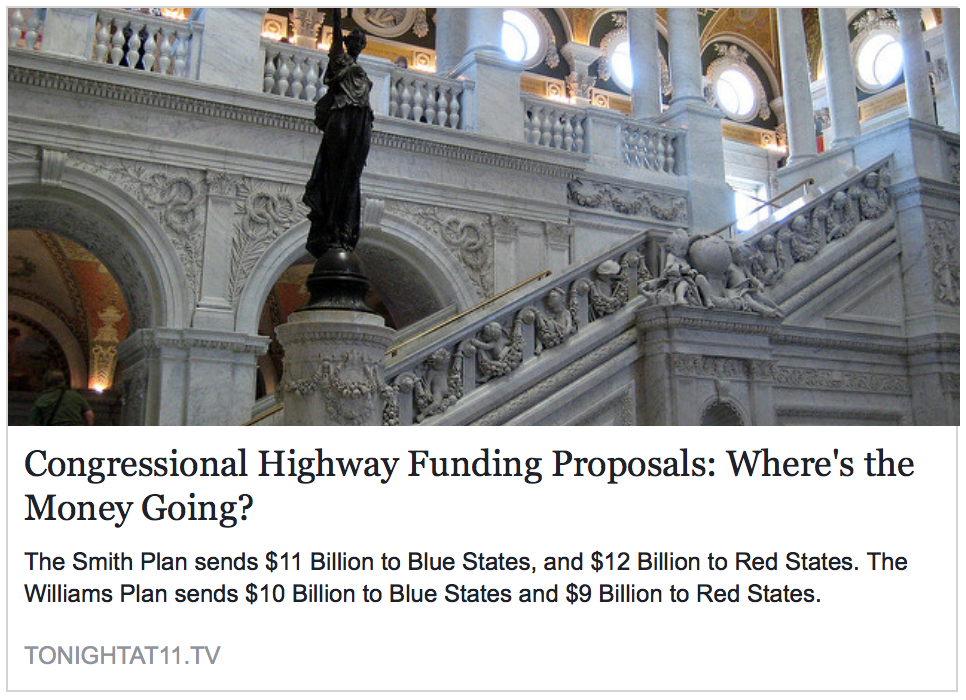
\includegraphics[width=.8\linewidth]{../data/highway_plan/Blue.png}
  \caption{Treatment Shown to Democrats}
  \label{fig:sfig1}
\end{subfigure}%
\begin{subfigure}{.5\textwidth}
  \centering
  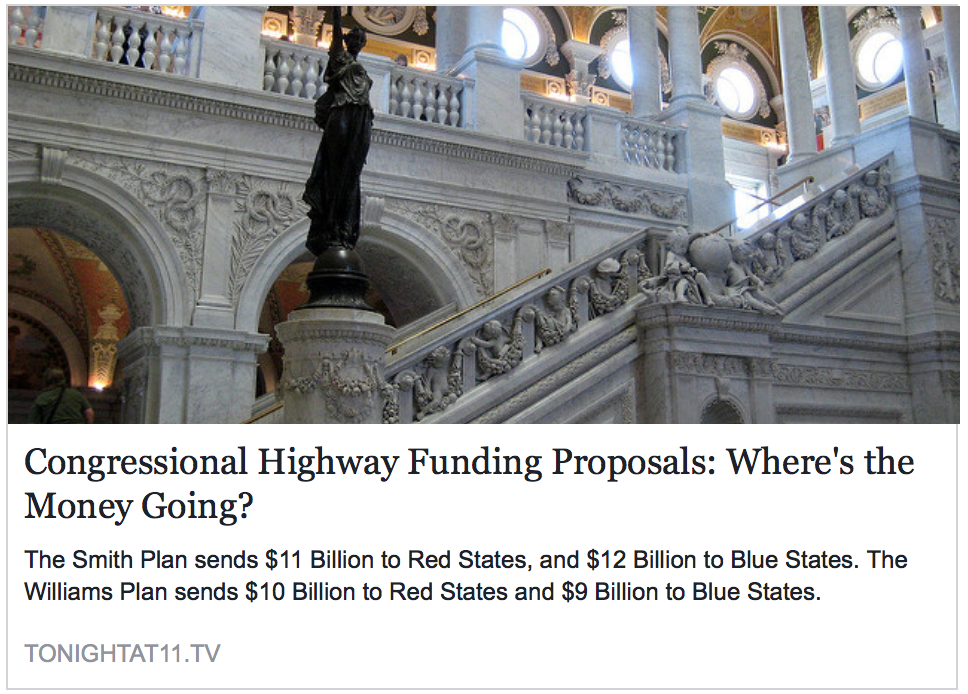
\includegraphics[width=.8\linewidth]{../data/highway_plan/Red.png}
  \caption{Shown to Republicans}
  \label{fig:sfig2}
\end{subfigure}
\caption{Vignettes}
\label{fig:fig}
\end{figure}

\section{Results}

As Table~\ref{tab:tab1} shows, two-third of the Democrats and three-fourths of the Republicans choose the Williams Plan rather than the Smith Plan.

% latex table generated in R 3.6.2 by xtable 1.8-4 package
% Tue Feb 18 19:56:19 2020
\begin{table}[h!]
\centering
\begin{tabular}{rrr}
  \toprule
 & Democrat & Republican \\ 
  \midrule
Smith Plan & 0.33 & 0.26 \\ 
  Williams Plan & 0.67 & 0.74 \\ 
   \bottomrule
\end{tabular}
\caption{Most Frequently Implicated Domains}
\label{tab:tab1}
\end{table}

\clearpage
\bibliographystyle{apsr}
\bibliography{pareto}

\end{document}